\section{Product Perspective}
\subsection{The world and the Machine}
\begin{figure}[H]
    \centering
    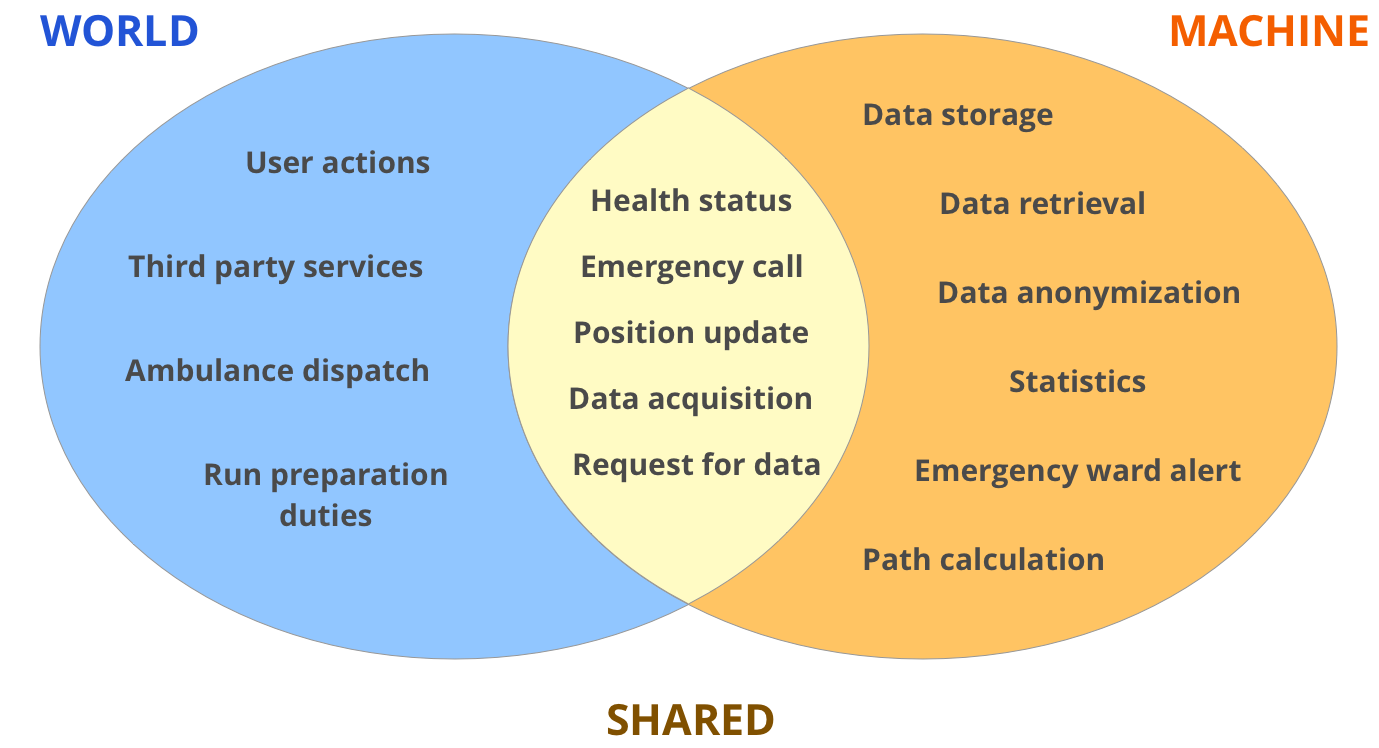
\includegraphics[scale=0.3]{rasdL/Pictures/worldmachine.png}

\end{figure}

\textbf{Some clarifications about the diagram:}\\ \\
The \underline{User actions} are all the behaviors that in the every day life the user performs in the world. The \underline{Third Party services} are all the services that will arise from the utilization and the study of the collected data. The \underline{Run preparation duties} are the efforts spent to planning and organizing a run event projected in the real world: e.g. block the circulation of vehicles for the run route that day and mark the run route. The \underline{Emergency ward alert} represents the background service that the machine performs to check the health status
of the users with AutomatedSos enabled. If it detects an anomalous state, triggers the Emergency procedure.

\newpage
\subsection{UML: Class Diagram}\\ \\
This is the UML model of  the whole system, based on a class diagram:
\begin{figure}[H]
    \centering
    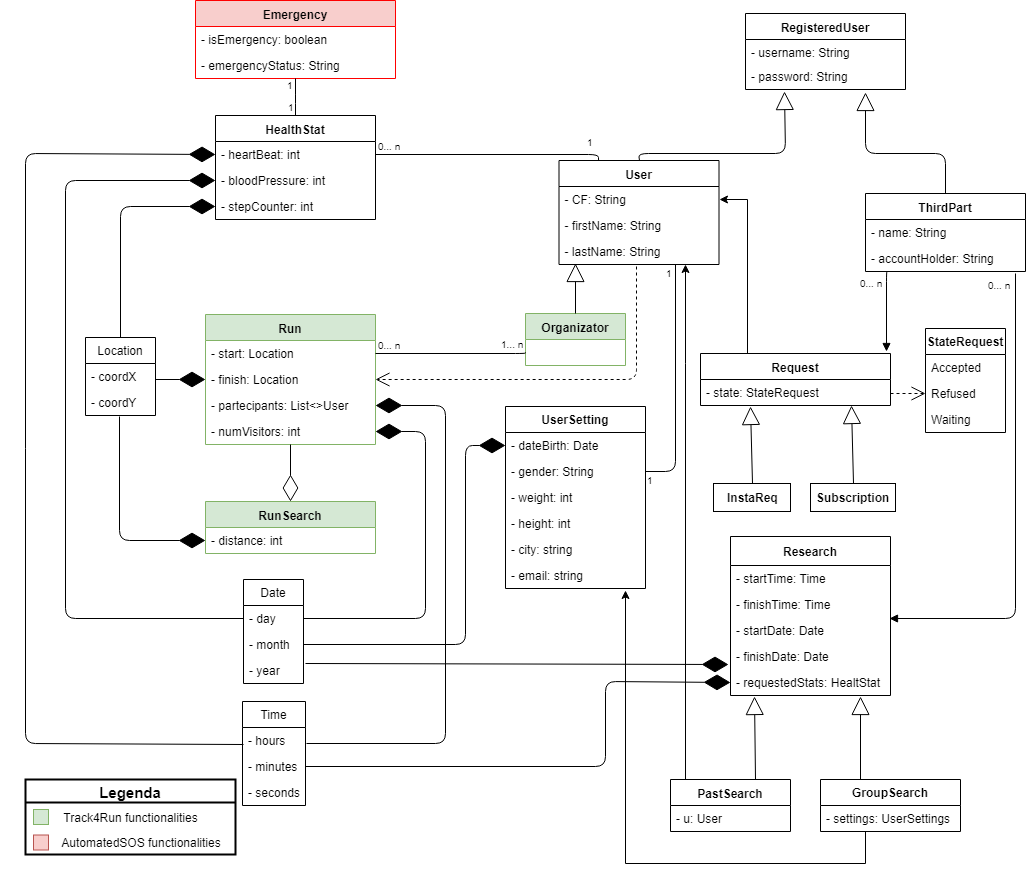
\includegraphics[scale=0.4]{Pictures/UML.png}

\end{figure}

\newpage
\subsection{State charts:}

\begin{figure}[H]
    \centering
    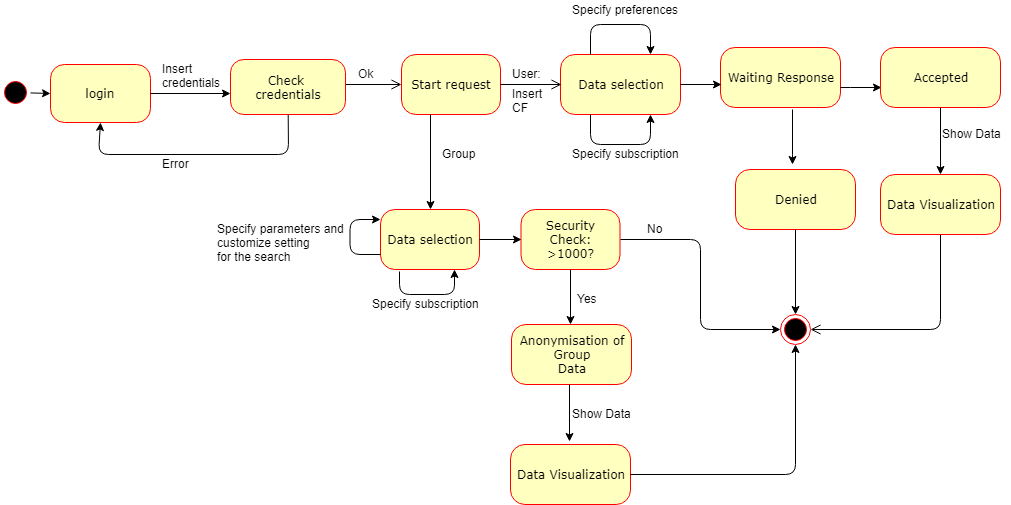
\includegraphics[scale=0.4]{Pictures/stateChart1.png}
    \caption{State chart of \emph{Data4Help} System}
\end{figure}

This is a background service that runs in order to keep track of the health status of each user, and notify the NHS in case of Emergency
\begin{figure}[H]
    \centering
    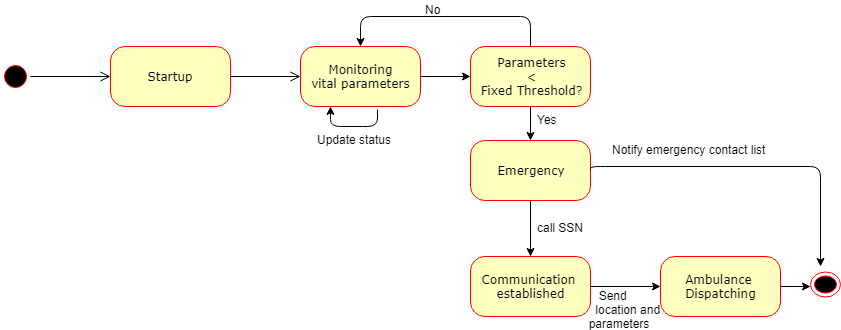
\includegraphics[scale=0.4]{Pictures/stateChart2.png}
    \caption{State chart of \emph{AutomatedSOS} System}
\end{figure}
\begin{figure}[H]
    \centering
    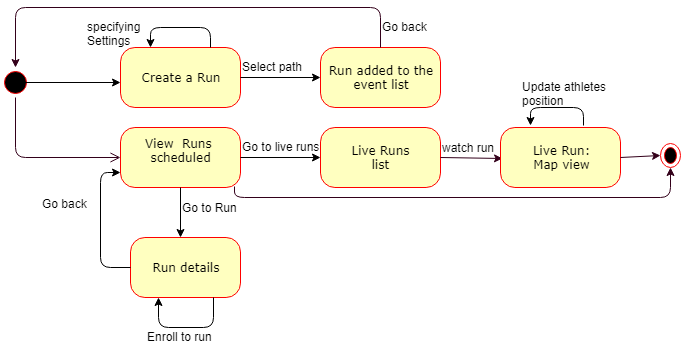
\includegraphics[scale=0.4]{Pictures/statechart3.png}
    \caption{State chart  of \emph{Track4Run} System}
\end{figure}
